\section{SYSTEM OVERVIEW}
\label{sec:system}
\subsection{Pattern prediction on a single stream}
%refine the stream and event pattern %
%define the pattern we deal formally%
% include base line 1 batch size in experemintal results%

For our work presented in this paper,
we use the approach presented in \cite{alevizos2017event}.
For the sake of self-containment,
we briefly describe this approach in the following,
first assuming that only a single stream is consumed
and then adjusting for the case of multiple streams.
We follow the terminology of \cite{luckham2008power,alevizos2015complex,zhou_pattern_2015} to formalize the problem we tackle.

\subsubsection{Problem formulation}

We define an input event and a stream of input events as follows:  
\begin{definition}
	Each event is defined as a tuple of attributes $e_i = (id,type,\tau,a_1,a_2.....,a_n)$, where $type$ is the event type attribute that takes a value from a set of finite event types/symbols $\Sigma$, $\tau$ represents the time when the event tuple was created,  the  $a_1,a_2,...,a_n$ are spatial or other contextual features (e.g., speed); these features are varying from one application domain to another. The attribute $id$ is a unique identifier that connects the event tuple to an associated domain object.
\end{definition}

\begin{definition}
A stream $s=\langle e_1,e_3,...,e_t,...\rangle$  is a time-ordered sequence of events.
\end{definition}

\par A user-defined pattern $\mathcal{P}$ is given in the form of a regular expression (i.e., using operators for \textit{sequence}, \textit{disjunction}, and \textit{iteration}) over $\Sigma$ (i.e., event types) \cite{alevizos2017event}.
More formally, a pattern is given through the following grammar:
\begin{definition}
$\mathcal{P} := E\ |\ \mathcal{P}_{1} ; \mathcal{P}_{2}\ | \mathcal{P}_{1} \vee \mathcal{P}_{2}\ |\ \mathcal{P}_{1}^{*}  $, where $E \in \Sigma$ is a constant event type. $;$ stands for sequence, $\vee$ for disjunction and $*$ for $\mathit{Kleene}-*$.
The pattern $\mathcal{P} := E$ is matched by reading an event $e_i$ iff $e_{i}.type = E$.
The other cases are matched as in standard automata theory.
\end{definition}


The problem at hand may then be stated as follows: given a stream $s$ of low-level events and a pattern $\mathcal{P}$, 
the goal is to estimate at each new event arrival the number of future events
that we will need to wait for until the pattern is satisfied (and therefore a full match is detected).

\subsubsection{Proposed approach}

As a first step, event patterns are converted to deterministic finite automata (DFA) through standard conversion algorithms.
As an example, see Figure ~\ref{fig:dfatcc} for the DFA of the simple sequential pattern $\mathcal{P}=a ; c ; c$ and an alphabet $\Sigma=\{a,b,c\}$
(note that the DFA has no dead states since we need to handle streams and not strings).
The next step is to derive a Markov chain that will be able to provide a probabilistic description of the DFA's run-time behavior.
\par Towards this goal, we use Pattern Markov Chains, as was proposed in \cite{nuel_pattern_2008}.
Under the assumption that the input events are independent and identically distributed (i.i.d.), it can be shown that there is a direct mapping of the states of the DFA to states of a Markov chain and the transitions of the DFA to transitions of the Markov chain.
\par The transition probabilities of the Markov chain are the occurrence probabilities of the various event types.
On the other hand, if the occurrence probabilities of the events are dependent on some of the previous events  seen in the stream (i.e., the stream is generated by an $m^{th}$ order Markov process), we might need to perform a more complex transformation 
(see \cite{nuel_pattern_2008} for details)
in order to obtain a ``proper'' Markov chain.
The transition probabilities are then conditional probabilities on the event types.
In any case,
we call such a derived Markov chain a Pattern Markov Chain (PMC) of order $m$
and denote by \pmcmr , where $\mathcal{P}$ is the initial pattern and $m$ the assumed order.
As an example, see Figure \ref{fig:mctcc1}, which depicts the PMC of order 1 for the generated DFA of Figure \ref{fig:dfatcc}.
%\begin{comment}
\begin{figure}[!ht]
\begin{centering}
\subfloat[\dfasr]{
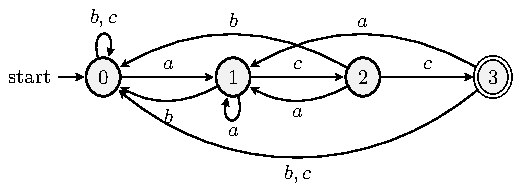
\includegraphics[width=0.35\textwidth]{./figures/forecasting/dfasr.pdf}
\label{fig:dfatcc}
}
\hfill
\subfloat[\pmconer]{
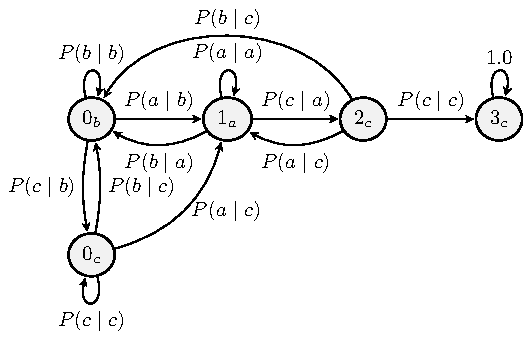
\includegraphics[width=0.35\textwidth]{./figures/forecasting/pmcr1.pdf}
\label{fig:mctcc1}
}
%\hfill
\caption{DFA and PMC for $\mathcal{P}=a ; c ; c$,  $\Sigma=\{a,b,c\}$, and order $m=1$  \cite{alevizos2017event}.}
\label{fig:dfa_mc_example}
\end{centering}
\end{figure}
%\end{comment}


\par After constructing a PMC, we can use it to calculate the so-called \textit{waiting-time} distributions.
Given a specific state of the PMC, a \textit{waiting-time} distribution gives us the probability of reaching a set of absorbing states in $n$ transition from now (absorbing states are states with self-loops and probability equal to $1.0$).
By mapping the final states of the initial DFA to absorbing states of the PMC
(see again Figure \ref{fig:dfa_mc_example}),
we can therefore calculate the probability of reaching a final state,
or, in other words, of detecting a full match of the original regular expression in $n$ events from now.

\par In order to estimate the final forecasts, another step is required,
since our aim is not to provide a single future point with the highest probability but an interval. 
Predictions are given in the form of intervals, like $I=(\mathit{start},\mathit{end})$. 
The meaning of such an interval is that the DFA is expected to reach a final state sometime in the future between $\mathit{start}$ and $\mathit{end}$ with probability at least some constant threshold $\theta_{fc}$ (provided by the user). 
These intervals are estimated by a single-pass algorithm that scans a waiting-time distribution and finds the smallest (in terms of length) interval that exceeds this threshold. 
An example is shown in Figure \ref{fig:wtdfas},
where the DFA in Figure \ref{fig:dfa1} is in state $1$,
the \textit{waiting-time} distributions for all of its non-final states are shown in Figure \ref{fig:wt1}
and the distribution, along with the prediction interval, for state $1$ are depicted in green.
\begin{figure}[!ht]
\begin{centering}
\subfloat[DFA, state 1.]{ 
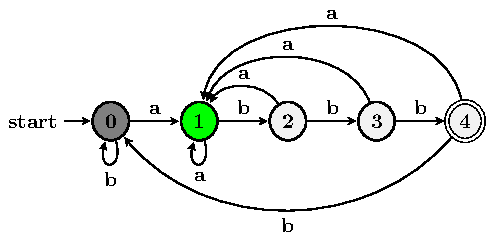
\includegraphics[width=0.19\textwidth]{./figures/forecasting/dfa1.pdf}
\label{fig:dfa1}
}
\subfloat[Waiting-time distribution, state 1.]{ 
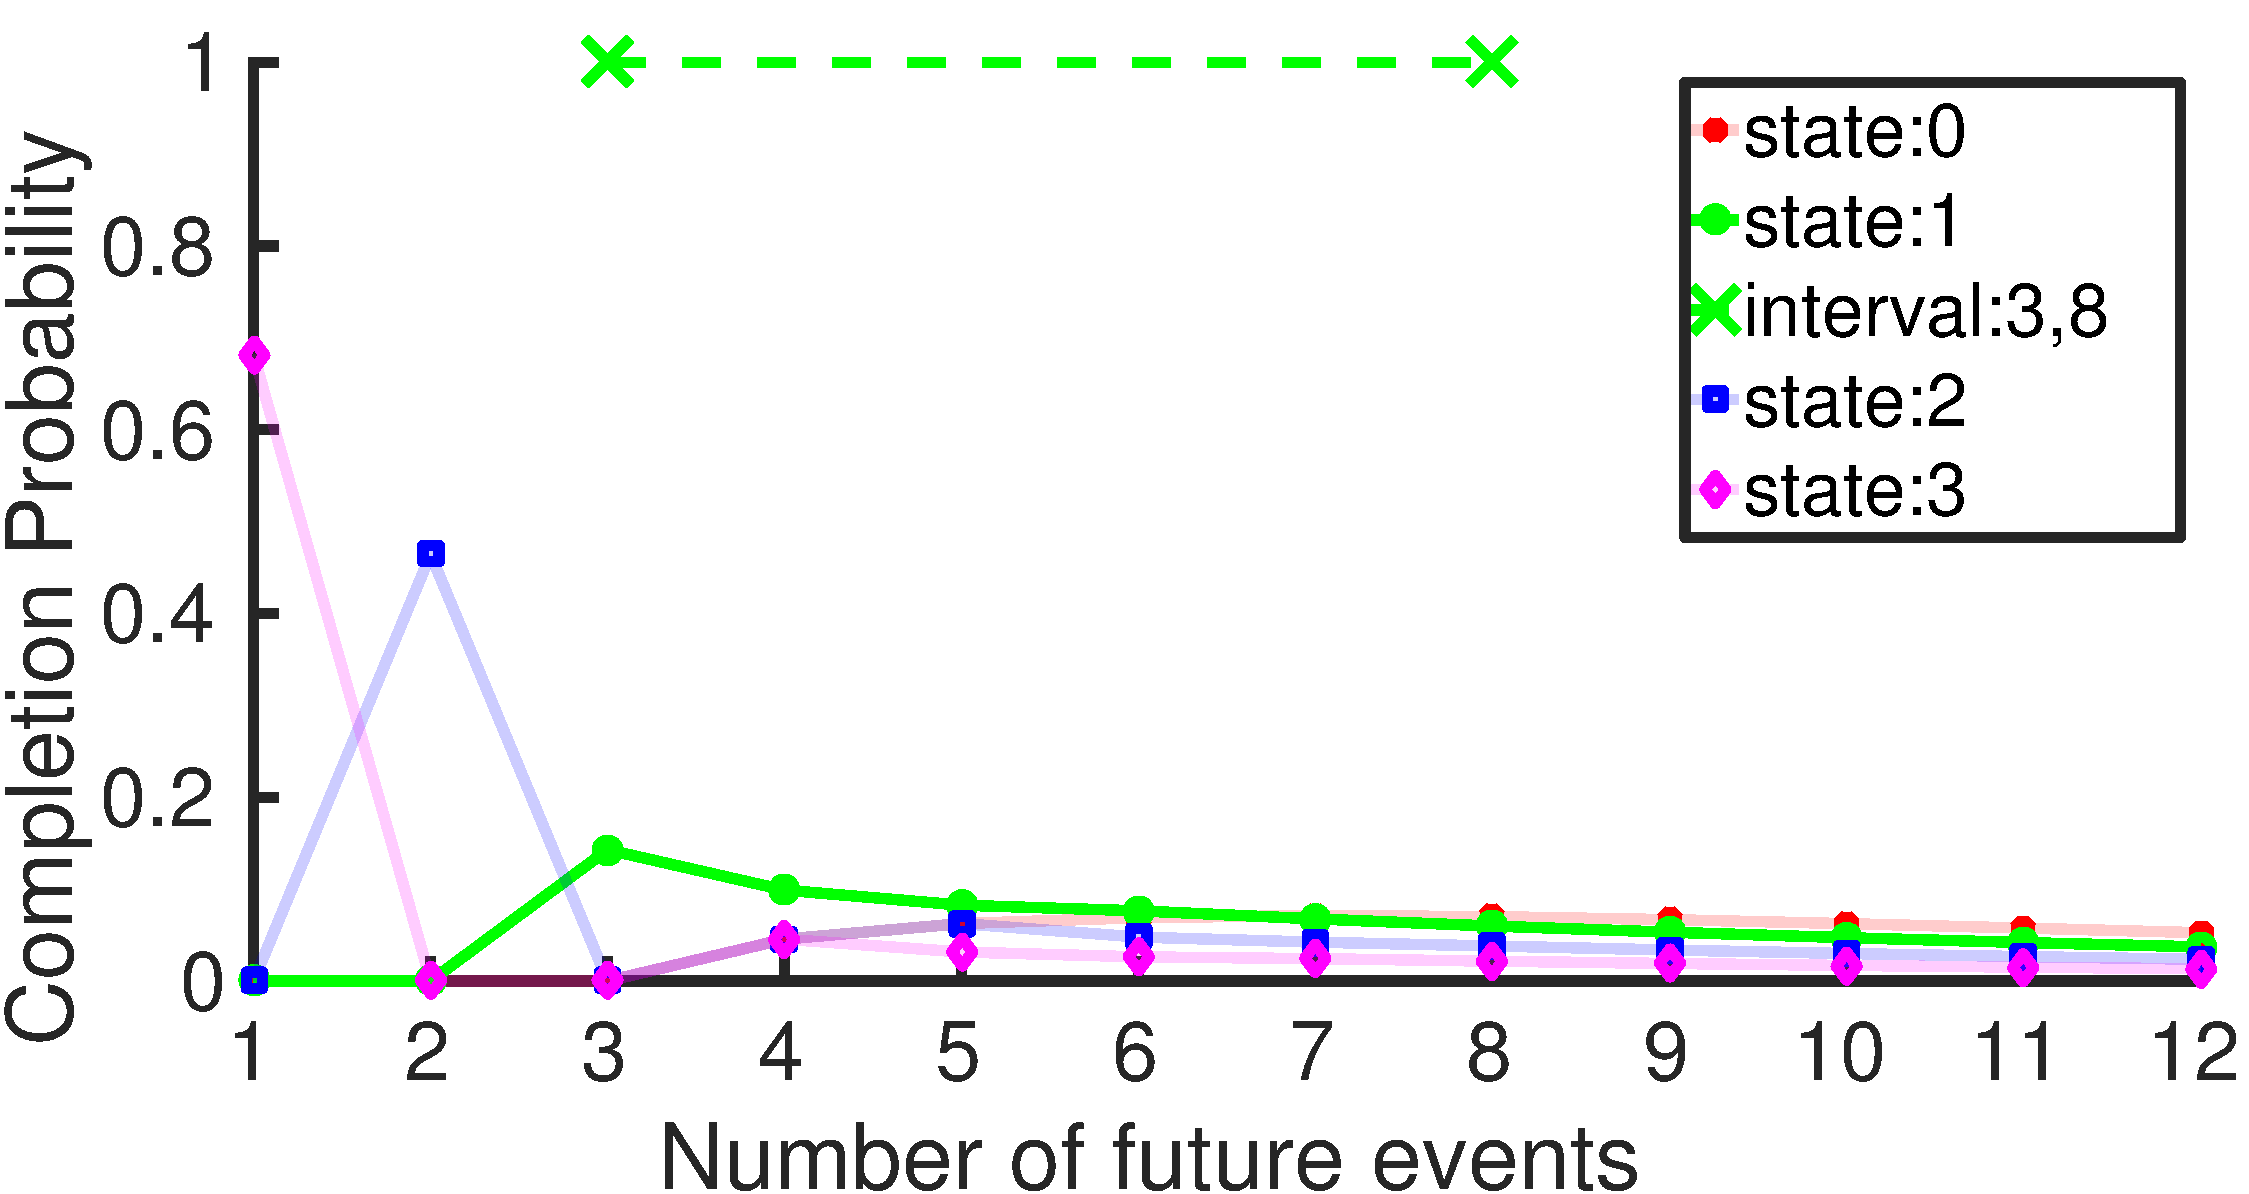
\includegraphics[width=0.28\textwidth]{./figures/forecasting/wt1.pdf}
\label{fig:wt1}
}
\caption{Example of how prediction intervals are produced. 
$\mathcal{P}=a ; b ; b ; b$, $\Sigma=\{a,b\}$, $m=1$, $\theta_{\mathit{fc}}=0.5$      \cite{alevizos2017event}.}
\label{fig:wtdfas}
\end{centering}
\end{figure}

The above described method assumes that we know the (possibly conditional) occurrence probabilities of the various event types appearing in a stream
(as would be the case with synthetically generated streams).
However, this is not always the case in real-world situations.
Therefore, it is crucial for a system implementing this method to have the capability to learn the values of the PMC's transition matrix.
One way to do this is to use some part of the stream to obtain the maximum-likelihood estimators for the transition probabilities. 
If $\boldsymbol{\Pi}$ is the transition matrix of a Markov chain with a set of states $Q$, 
$\pi_{i,j}$ the transition probability from state $i$ to state $j$,
$n_{i,j}$ the number of observed transitions from state $i$ to state $j$,
then the maximum likelihood estimator for $\pi_{i,j}$ is given by:
\begin{equation*}
\label{eq:pi_estim}
\hat{\pi}_{i,j}=\frac{n_{i,j}}{\sum_{k \in Q} n_{i,k}}=\frac{n_{i,j}}{n_{i}}
\end{equation*}
Executing this learning step on a single node might require a vast amount of time until we arrive at a sufficiently good model.
In this paper, we present a distributed method for learning the transition probability matrix.

\subsection{Pattern prediction on multiple streams}

\subsubsection{Problem formulation}
Let $O = \{ o_1, ..., o_k\}$ be a set of \emph{$K$}  objects (i.e., moving objects) 
and $S = \{ s_1, ..., s_k\}$ a set of real-time streams of events,
where $s_i$ is generated by the object $o_i$.
Let $\mathcal{P}$ be a user-defined pattern which we want to apply to every stream $s_i$,
i.e., each object will have its own DFA.

\par The setting that is considered in this work is then described in the following:
we have \emph{$K$} input event streams $S$ and a system consisting of \emph{$K$} distributed predictor nodes $n_1,n_2...,n_k$, each of which consumes an input event stream $s_i\in S$. The goal is to provide timely predictions and be able to do this at large-scale.
Each node $n_i$ handles a single event stream $s_i$ associated with a moving object $o_i \in O$. In addition,  it  maintains a local prediction model $f_i$ for the user-defined pattern $\mathcal{P}$. The $f_i$ model provides the online prediction about the future full match of the pattern $\mathcal{P}$ in $s_i$  for each new arriving event tuple. 
\par In short, we have multiple running instances of an online prediction algorithm on distributed nodes for multiple input event streams. More specifically, the input to our system consists of massive streams of events  that describe trajectories of moving vessels in the context of maritime surveillance, where there is one predictor node for each vessel's event stream.
  
%
%The defined pattern $\mathcal{P}$ is monitored over each event stream $s_i$  by a  predictor nodes  $n_i$  that maintains a local prediction model $f_i$, where there is one node for each vessel's event stream.  The prediction model $f_i$ gives the ability to provide an online predictions about when the pattern will be completed in the form of an expected number of future events before a full match does occur.

\subsubsection{The proposed approach}
\label{sec:proposed_approach}
\par We designed and developed a scalable and distributed patterns prediction system over a massive input event streams of moving objects. As the base prediction model, we use the PMC forecasting method \cite{alevizos2017event}. Moreover,  we propose to enable the information exchange between the distributed predictors/learners of the input event streams, by adapting the distributed online prediction protocol of \cite{kamp2014communication} to synchronize the prediction models, i.e., the transitions probabilities matrix of the PMC predictors.

\par Algorithm~\ref{algonline:dol} presents the distributed online prediction protocol by dynamic model synchronization on both the predictor nodes and the coordinator. We refer to the PMC's transition matrix $\boldsymbol{\Pi}_i$ on predictor node $n_i$ by $f_i$. That is, when a predictor $n_i:\ i \in[k]$ observes an event $e_j$ it revises its internal model state (i.e., $f_i$) and provides a prediction report. Then it checks the local conditions  (batch size $b$ and local model divergence from a reference model $f_r$) to decide whether there is a need to synchronize its local model with the coordinator [or not].  $f_r$ is maintained in the predictor node as a copy of the last computed aggregated model $\hat{f}$ from the previous full synchronization step, which is shared between all local predictors/learners. By monitoring the local condition $\|f_i - f_r\|^2 > \Delta$ on all local predictors, we have a guarantee that if none of the local conditions is violated, the divergence (i.e., variance of local models $\delta(f)=\frac{1}{k} \sum_{j=1}^{k}\|f_i - \hat{f}\|^2$) does not exceed the threshold $\Delta$ \cite{kamp2014communication}. 

\par On the other hand, the coordinator receives the prediction models from the predictor nodes that requested for model synchronization (violation). Then it tries to keep incrementally querying other nodes for their local prediction models until reaching out all nodes, or the variance of the aggregated model $\hat{f}$ that is computed from the already received models less or equal than the divergence threshold  $\Delta$. Finally, the aggregated model $\hat{f}$ is sent back to the predictor nodes that sent their models after the violation or have been queried by the coordinator.

\begin{algorithm}[h]
	\caption{Communication-efficient Distributed Online Learning Protocol } 
	\begin{algorithmic}[1] 
		\Statex \Indm  \textbf{Predictor} node $n_i$: at observing event $e_j$
		\Statex \Indp update the prediction model parameters $f_i$ and provide a prediction service \; 

		\Statex \If {$j\mod b = 0\ and\ \|f_i - f_r\|^2 > \Delta$}  
		\Statex send  $f_i$ to the Coordinator (violation) \;
		\Statex \Indm \textbf{Coordinator}:
		\Statex \Indp receive local models with violation 
		 $B=\{f_i\}_{i=1}^m$ \;
	
	
		\Statex \While{$|B| \neq k $ and $\frac{1}{|B|} \ \sum_{f_i\in  \Pi}\|f_i - \hat{f}\|^2 > \Delta$}{
			
			 \Statex  \hspace{\algorithmicindent} add other nodes have not reported violation for \Statex \hspace{\algorithmicindent} their models $ B \gets \{f_l : f_l \notin B\ and\ l \in [k]\}$    \;
			\Statex  \hspace{\algorithmicindent} receive models from nodes add to $B$\;
	}
        \Statex
		\Statex compute a new global model $\hat{f}$ \;
		\Statex send $\hat{f}$ to all the predictors in $B$ and set $f_{1}\dots f_{m}=\hat{f} $\; 
		\Statex \If {$|B| = k$}{
		\Statex  \hspace{\algorithmicindent} set a new reference model $f_r	\gets \hat{f}$ \; }
	
	\end{algorithmic}
	\label{algonline:dol}
\end{algorithm}


\par This protocol was introduced for linear models, and has been  extended to handle kernelized online learning models \cite{kamp2016communication}. We also employ this protocol for the pattern prediction model, which is internally based on the PMC \pmcmr. This allows the distributed \pmcmr\ predictors for multiple event streams to  synchronize their models (i.e., the transition probability matrix of each predictor) within the system in a communication-efficient manner. 



\par We propose a \textit{synchronization operation} for the parameters of the models ($f_i=\boldsymbol{\Pi}_i :i \in[k]$) of the $k$ distributed PMC predictors. The operation is based on distributing the maximum-likelihood estimation \cite{anderson1957statistical} for the transition probabilities of the underlying \pmcmr\ models described by: 
\begin{equation*}
\label{eq:dis_pi_estim}
\hat{\pi}_{i,j}=\frac{\sum_{k \in K} n_{k,i,j}}{\sum_{k \in K} \sum_{l \in L} n_{k,i,l}}
\end{equation*}

\par Moreover, we measure the divergence of local models from the reference model  $\|f_k - f_r\|^2$ by calculating the sum of square difference between the transition probabilities  $\boldsymbol{\Pi}_i$ and  $\boldsymbol{\Pi}_r$:
\begin{equation*}
\label{eq:dis_pi_varinace}
\|f_k - f_r\|^2=\sum_{i,j} (\hat{\pi}_k{i,j} -\hat{\pi}_r{i,j})^2
\end{equation*}
\par In general, our approach relies on enabling the collaborative learning between the prediction models of  the input event streams. By doing so, we assume that the underlying event streams belong to the same  distribution and share the same behavior (e.g., mobility patterns). We claim this assumption is reasonable in many application domains: for instance, in the context of maritime surveillance, vessels travel through standard routes, defined by the International Maritime Organization (IMO). Additionally, vessels have similar mobility patterns in specific areas such as moving with low speed and multiple turns near the ports \cite{pallotta2013vessel,liu2014knowledge}. That allows our system to construct a coherent global prediction model dynamically for all input event streams based on merging their local prediction models.

% may add it to conclusion 
%\par By enabling collaborative learning our approach is imposing an acceleration of learning of the underlying prediction models with less training data, in addition, it provides an improvement of the predictive performance compared to the no-distributed  version of event forecasting with Pattern Markov Chains system. 


\subsection{Distributed architecture}
\label{sec:architecture}
Our system consumes as an input\footnote{In practice, the aggregated input events stream is composed of multiple event streams (partitions) from a set of moving objects.} an aggregated stream of events coming from a large number of moving objects, which is continuously collected and fed into the system. It allows users to register a pattern $\mathcal{P}$ to be monitored over each event stream of a moving object. The output stream consists of original input events and predictions of full matches of $\mathcal{P}$, displayed to the end users. Figure ~\ref{fig:architecture} presents the overview of our system architecture and its main components.      


\begin{figure}[h]

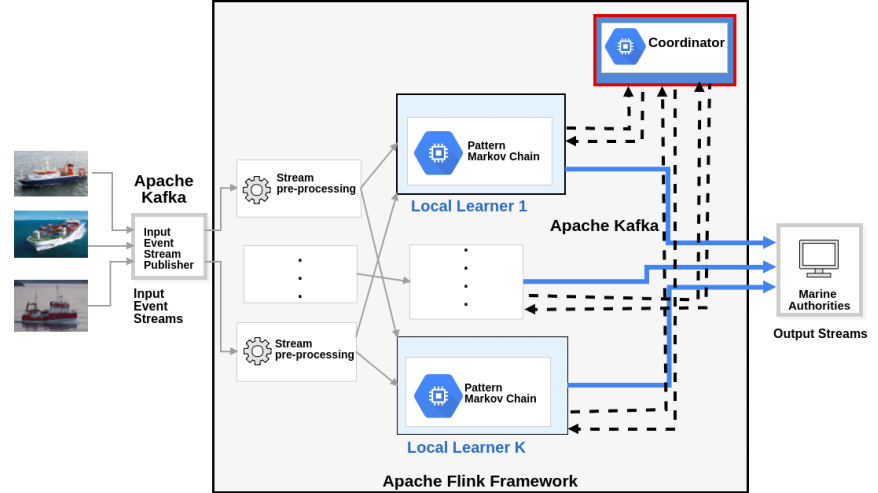
\includegraphics[width=\linewidth]{figures/distributed_architecture_2.png}
	
\caption{System Architecture.}
\label{fig:architecture}
\end{figure}

The system is composed of three processing units:   \begin{enumerate*}[(i)]
	\item pre-processing operators that receive the input event stream and perform filtering and ordering operations, before partitioning the input event stream to multiple event streams based on the associated moving object 
	\item predictor nodes (learners), which are responsible for maintaining a prediction model for the input event streams. Each prediction node is configured to handle an event stream from the same moving object, in order to provide online predictions for a predefined pattern $\mathcal{P}$  
	\item a coordinator node that communicates through Kafka stream channels with the predictors to realize the distributed online learning protocol. It builds a global prediction model, based on the received local models, and then shares it among the predictors.
\end{enumerate*}

\par Our distributed system consists of multiple pre-processing operators, prediction nodes, and a central coordinator node. All units run concurrently and are arranged as a  data processing pipeline, depicted in Figure ~\ref{fig:architecture}. We leverage Apache Kafka as a messaging platform to ingest the input event streams and to publish the resulting streams. Also, it is used as the communication channel between the predictor nodes and the coordinator. Apache Flink is employed to execute the system's distributed processing units over the input event streams: the pre-processing operators,  the prediction units, and the coordinator node. Our system architecture can be modeled as a logical network of processing nodes, organized in the form of a DAG, inspired by the Flink runtime dataflow programs \cite{carbone2015apache}.  
